% Prepared by Calvin Kent
\documentclass[12pt,oneside]{book} %
\usepackage{CKpreamble}
\usepackage{CKlecture}
\usepackage{mdframed}
\usepackage{import}
\usepackage{pdfpages}
\usepackage{euscript}
\usepackage{transparent}
\usepackage{xcolor}
\usepackage{tasks}
\usepackage{tkz-euclide}


\newcommand{\incfig}[2][1]{%
    \def\svgwidth{#1\columnwidth}
    \import{./figures/}{#2.pdf_tex}
}


\newcounter{step}[section]
\newenvironment{step}[1][]
{\refstepcounter{step} \textit{Step #1.}}

\newcounter{Rule}[section]
\newenvironment{Rule}[1][]
{\refstepcounter{Rule} \textit{Rule #1.}}


\pdfsuppresswarningpagegroup=1

%
\renewcommand*{\doctitle}{Class Based Lecture Notes}
\makeatletter\patchcmd{\chapter}{\if@openright\cleardoublepage\else\clearpage\fi}{}{}{}\makeatother % only used in class based
\begin{document}
	% Start of Class settings
	\renewcommand*{\term}{Term 2} % Term
	\renewcommand*{\coursecode}{MCR3U} % Course code
	\renewcommand*{\coursename}{Course Name} % Full course name
	\renewcommand*{\thelecnum}{8} % Lecture number
	\renewcommand*{\profname}{Prof Name} % Prof Name
	\renewcommand*{\colink}{http://www.student.math.uwaterloo.ca/~c2kent} % Course outline link
	% End of Class settings
	\clearpage
	\pagenumbering{arabic}
	\pagestyle{classlecture}
	%%% Note to user: CTRL + F <CHANGE ME:> (without the angular brackets) in CKpreamble to specify graphics paths accordingly.
	%%% If a new chapter was started in the middle of a lecture, \fix chap{Second Chapter} must be used immediately above the next lecture.
	% Course notes start
\setchap{8}{Trigonometry Part I}
\begin{lec}{January 2022}
	\chapter{\chapname\chaplec}

  Trigonometry is concerned with the study of the so called \textit{Unit circle}. Before jumping in, lets recall
  some of the notation and terminology we'll be dealing with.
  
  \begin{defn}
      Given a right triangle,

  \begin{center}
    \begin{tikzpicture}
    %coordinate system

    \draw[black] (5,1) -- (5,5) node[circle,red,fill,inner sep=2pt]{} node[above]{$B$};
    \draw[black] (0,1) -- (5,1) node[circle,black,fill,inner sep=2pt]{} node[below]{$C$};
    \draw[black] (0,1) node[circle,black,fill,inner sep=2pt]{} node[below]{$A$};
    \draw (4.7,1) |- ++(0.3,0.3);
    \draw[black] (0,1) -- (5,5) node[circle,black,fill,inner sep=2pt]{} node[above]{$B$};
    \draw (1,1) arc (0:38:1)node[midway,above right]{$\theta$};
    \end{tikzpicture}
  \end{center}

  \textbf{Relative} to the angle $\theta$, we define the following sides of the triangle,
      \begin{itemize}
        \item \textbf{Adjacent side:} The side with both the angle $\theta$ and the right angle. (Side
          $\textbf{AC}$ in fig)
        \item \textbf{Hypotenuse side:} The side opposite to the right angle. (Side
          $\textbf{AB}$ in fig)
        \item \textbf{Opposite side:} The remaining side. (Side
          $\textbf{BC}$ in fig)
      \end{itemize}

  \end{defn}

  \begin{rem}
      Notice how in the definition I emphasize that the way we label these sides are relative to the position of
      the angle $\theta$. How we label the adjacent, opposite and hypotenuse will change depending on the specified
      angle.
  \end{rem}

  \begin{ex}
    Identify the Adj, Opp, Hyp sides for the following triangles \textit{relative} to the angle $\gamma$.
    \begin{tasks}(2)
      \task \texttt{  }\\
          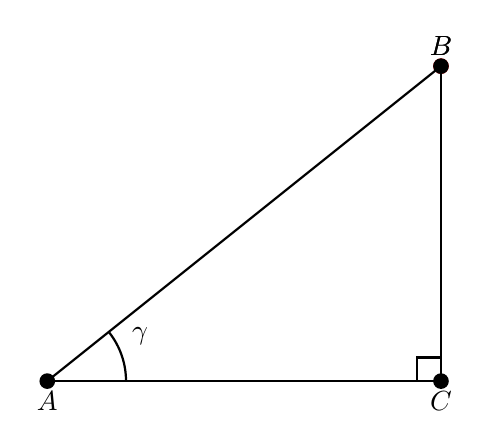
\begin{tikzpicture}[thick]
          %coordinate system

          \draw[black] (5,1) -- (5,5) node[circle,red,fill,inner sep=2pt]{} node[above]{$B$};
          \draw[black] (0,1) -- (5,1) node[circle,black,fill,inner sep=2pt]{} node[below]{$C$};
          \draw[black] (0,1) node[circle,black,fill,inner sep=2pt]{} node[below]{$A$};
          \draw (4.7,1) |- ++(0.3,0.3);
          \draw[black] (0,1) -- (5,5) node[circle,black,fill,inner sep=2pt]{} node[above]{$B$};
          \draw (1,1) arc (0:38:1)node[midway,above right]{$\gamma$};
          \end{tikzpicture}

      \task \texttt{(**)}\\
          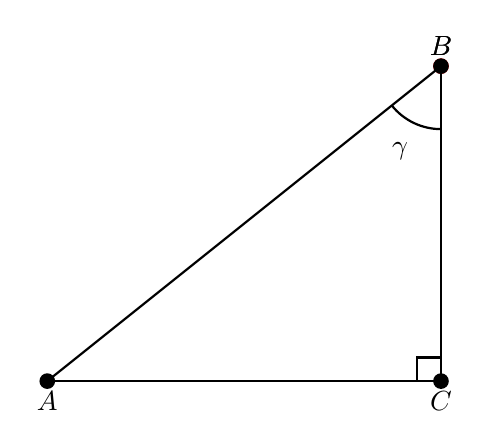
\begin{tikzpicture}[thick]
          \coordinate (A) at (0,1);
          \coordinate (B) at (5,5);
          \coordinate (C) at (5,1);

          \draw[black] (5,1) -- (5,5) node[circle,red,fill,inner sep=2pt]{} node[above]{$B$};
          \draw[black] (0,1) -- (5,1) node[circle,black,fill,inner sep=2pt]{} node[below]{$C$};
          \draw[black] (0,1) node[circle,black,fill,inner sep=2pt]{} node[below]{$A$};
          \draw (4.7,1) |- ++(0.3,0.3);
          \draw[black] (0,1) -- (5,5) node[circle,black,fill,inner sep=2pt]{} node[above]{$B$};

          \tkzMarkAngle[fill= orange,size=0.8cm,%
          opacity=1](A,B,C)
          \tkzLabelAngle[pos = 1.2](A,B,C){$\gamma$}

          \end{tikzpicture}

    \end{tasks}

    \newpage

  \end{ex}

  \section{Primary Trigonometric Ratio's}
  \begin{defn}
      Given a right triangle and an inscribed angle $\theta$, we define the \textbf{primary trigonometric ratio's}
      to be,
      \[
          \sin \theta = \frac{\textbf{Adjacent}}{\textbf{Hypotenuse}}\,\,\,\,\,\,\,
          \cos \theta = \frac{\textbf{Opposite}}{\textbf{Hypotenuse}}\,\,\,\,\,\,\,
          \tan \theta = \frac{\textbf{Opposite}}{\textbf{Adjacent}}\,\,\,\,\,\,\,
      \] 
  \end{defn}

  \begin{thrm}[Pythagorean's Theorem] Given a right triangle, the following holds,
    \[
          \left( \textbf{Hypotenuse} \right) ^2 = \left( \textbf{Adjacent} \right) ^2 + 
                                          \left( \textbf{Opposite} \right) ^2
    .\] 
    
  \end{thrm}

  \begin{ex}
    Compute the primary trigonometric ratios of the angle $\theta$.
    
    \begin{tasks}(2)
      \task \texttt{  }\\
          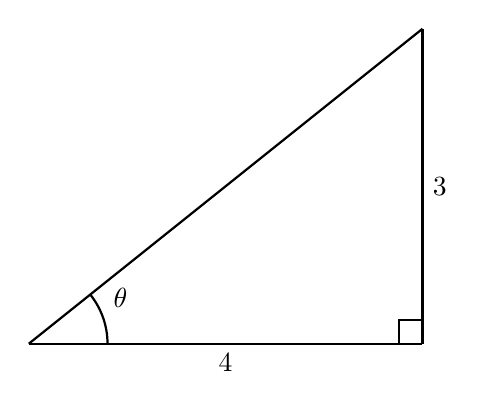
\begin{tikzpicture}[thick]
          %coordinate system

          \draw[black] (5,1) -- (5,5) node[midway,right]{$3$};
          \draw[black] (0,1) -- (5,1) node[below,midway]{$4$};
          \draw (4.7,1) |- ++(0.3,0.3);
          \draw[black] (0,1) -- (5,5);
          \draw (1,1) arc (0:38:1)node[midway,above right]{$\theta$};
          \end{tikzpicture}

      \task \texttt{(**)}\\
          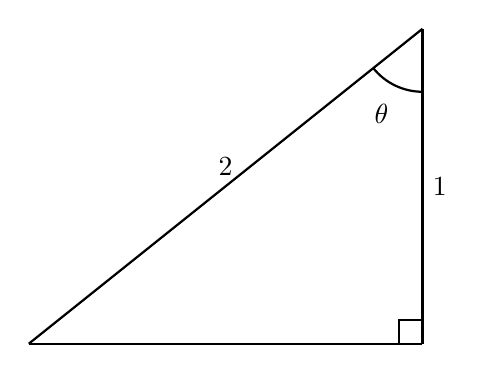
\begin{tikzpicture}[thick]
          \coordinate (A) at (0,1);
          \coordinate (B) at (5,5);
          \coordinate (C) at (5,1);

          \draw[black] (5,1) -- (5,5) node[midway, right]{$1$};
          \draw[black] (0,1) -- (5,1);
          \draw (4.7,1) |- ++(0.3,0.3);
          \draw[black] (0,1) -- (5,5) node[midway, above]{$2$};

          \tkzMarkAngle[fill= orange,size=0.8cm,%
          opacity=1](A,B,C)
          \tkzLabelAngle[pos = 1.2](A,B,C){$\theta$}

          \end{tikzpicture}

    \end{tasks}
  \end{ex}

  We can also use the primary trigonometric ratios to help solve for unknown sides in a right triangle. Get \textbf{
  your calculator} ready. Henceforth I will be describing triangles more concisely using syntactical representations
  that conveniently preserve our semantics.


  \begin{ex} \texttt{  }
    \begin{enumerate}[label=(\alph*)]
      \item Let $\triangle ABC$ be a \textbf{right triangle} with  angle $\angle ACB = 40^{\circ}$ and
        \textit{opposite side} $AB = 4$ relative to $\angle ACB$. Determine the length of sides $CB$ and $CA$.
      \item Let $\triangle FGH$ be a \textbf{right triangle} with angle $\angle FHG = 35^{\circ}$ and
        \textit{hypotenuse} $FH = 7$. Determine the length of sides $FG$ and $HG$. \hfill \texttt{(**)}
    \end{enumerate}
  \end{ex}

  There are a group of triangles that form convenient trigonometric ratios that are referred to as the \textbf{special
  triangles}. Their convenience lies within the fact that you \textbf{don't} have to resort to your calculator because
  they form nice ratios.

  \newpage

  \begin{thrm}[Special Triangle's]
    We define the \textbf{special triangle's} to be,

    \begin{tasks}(2)
      \task \texttt{  }\\
          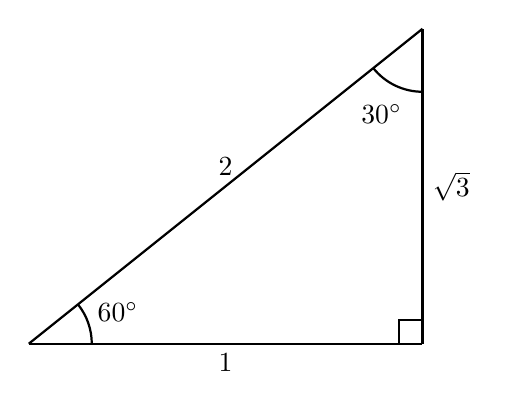
\begin{tikzpicture}[thick]
          \coordinate (A) at (0,1);
          \coordinate (B) at (5,5);
          \coordinate (C) at (5,1);

          \draw[black] (5,1) -- (5,5) node[midway, right]{$\sqrt{3}$};
          \draw[black] (0,1) -- (5,1) node[midway, below]{$1$};
          \draw (4.7,1) |- ++(0.3,0.3);
          \draw[black] (0,1) -- (5,5) node[midway, above]{$2$};

          \tkzMarkAngle[fill= orange,size=0.8cm,%
          opacity=1](A,B,C)
          \tkzLabelAngle[pos = 1.2](A,B,C){$30^{\circ}$}

          \tkzMarkAngle[fill= orange,size=0.8cm,%
          opacity=1](C,A,B)
          \tkzLabelAngle[pos = 1.2](C,A,B){$60^{\circ}$}

          \end{tikzpicture}

      \task \texttt{  }\\
          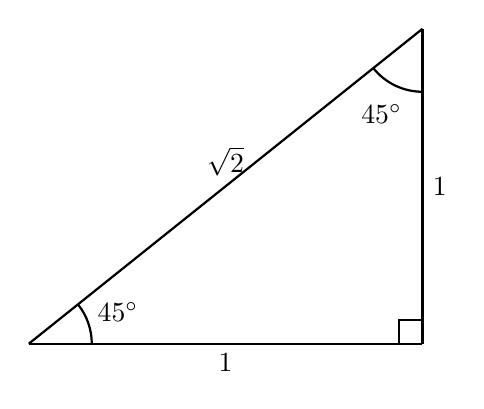
\begin{tikzpicture}[thick]
          \coordinate (A) at (0,1);
          \coordinate (B) at (5,5);
          \coordinate (C) at (5,1);

          \draw[black] (5,1) -- (5,5) node[midway, right]{$1$};
          \draw[black] (0,1) -- (5,1) node[midway, below]{$1$};
          \draw (4.7,1) |- ++(0.3,0.3);
          \draw[black] (0,1) -- (5,5) node[midway, above]{$\sqrt{2}$};

          \tkzMarkAngle[fill= orange,size=0.8cm,%
          opacity=1](A,B,C)
          \tkzLabelAngle[pos = 1.2](A,B,C){$45^{\circ}$}

          \tkzMarkAngle[fill= orange,size=0.8cm,%
          opacity=1](C,A,B)
          \tkzLabelAngle[pos = 1.2](C,A,B){$45^{\circ}$}

          \end{tikzpicture}

    \end{tasks}
    And define the corresponding \textbf{special angles} to be,
      \[
          \sin 45^{\circ} = \frac{1}{\sqrt{2}}\,\,\,\,\,\,\,
          \cos 45^{\circ} = \frac{1}{\sqrt{2}}\,\,\,\,\,\,\,
          \tan 45^{\circ} = 1\,\,\,\,\,\,\,
      \]

      \[
          \sin 60^{\circ} = \frac{\sqrt{3}}{2}\,\,\,\,\,\,\,
          \cos 60^{\circ} = \frac{1}{2}\,\,\,\,\,\,\,
          \tan 60^{\circ} = \sqrt{3} \,\,\,\,\,\,\,
          \\
      \]

      \[
          \sin 30^{\circ} = \frac{1}{2}\,\,\,\,\,\,\,
          \cos 30^{\circ} = \frac{\sqrt{3}}{2}\,\,\,\,\,\,\,
          \tan 30^{\circ} = \frac{1}{\sqrt{3} }\,\,\,\,\,\,\,
          \\
      \] 
  \end{thrm}

  \begin{ex}
    \texttt{  }
    \begin{enumerate}[label=(\alph*)]
      \item Let $\triangle PQR$ be a \textbf{right triangle} with angle $\angle PQR = 60^{\circ}$ and 
        \textit{hypotenuse} $PQ = 4$. Determine the length of the sides $QR$ and $PR$.\hfill \texttt{(**)}
      \item Determine the value of,
        \[
              \sin 60^{\circ}\cdot \tan 60^{\circ} + \cos 60^{\circ}\cdot \sin 30^{\circ}
        .\] 
    \end{enumerate}
  \end{ex}

  \subsection{Inverse trigonometric functions}
  In turns out that each of $\sin \theta$, $\cos \theta$, $\tan \theta$ are invertible and have inverse functions that
  can give us the value of an inscribed angle provided we already have knowledge of any of the three primary corresponding
  ratio's.

  \begin{defn}
    For each of $\sin \theta$, $\cos \theta$, $\tan \theta$ we define their inverse functions to be,
    \[
          \theta =  \sin^{-1}\left(\frac{\textbf{Adjacent}}{\textbf{Hypotenuse}}\right)\,\,\,\,\,\,\,
          \theta =\cos^{-1} \left(\frac{\textbf{Opposite}}{\textbf{Hypotenuse}}\right)\,\,\,\,\,\,\,
          \theta = \tan^{-1}\left( \frac{\textbf{Opposite}}{\textbf{Adjacent}}\right)\,\,\,\,\,\,\,
    .\] 
  \end{defn}

  \newpage

  \begin{ex} \texttt{  }
    \begin{enumerate}[label=(\alph*)]
      \item Let $\triangle PQR$ be a \textbf{right triangle} with $PQ = 5$ and $QR = 3$. Determine
        the measure of the angle $\angle PQR$ and $\angle QPR$.
      \begin{center}
          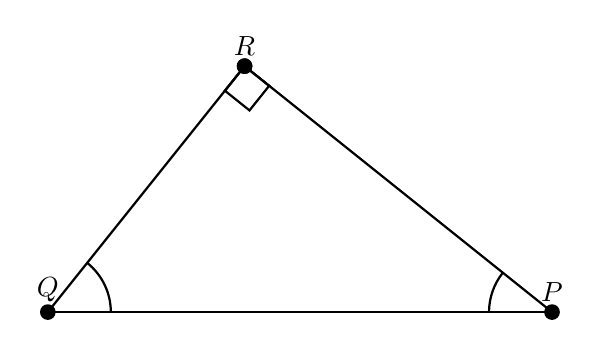
\begin{tikzpicture}[thick]
          \coordinate (Q) at (0,2);
          \coordinate (R) at (2.49878019,5.123475);
          \coordinate (P) at (6.403124,2);

          \draw[black] (0,2) -- (6.403124,2) node[circle,fill,inner sep=2pt]{} node[above]{$P$};
          \draw[black] (0,2) -- (2.49878019,5.123475) node[circle,black,fill,inner sep=2pt]{} node[above]{$R$};
          \draw[black] (6.403124,2) -- (2.49878019,5.123475) node[circle,black,fill,inner sep=2pt]{};
          \draw[black] (0,2) node[circle,black,fill,inner sep=2pt]{} node[above]{$Q$};

          \tkzMarkRightAngle[size=0.4,opacity=1](Q,R,P)% square angle here

          \tkzMarkAngle[fill= orange,size=0.8cm,%
          opacity=1](P,Q,R)
          \tkzLabelAngle[pos = 1.2](P,Q,R){}

          \tkzMarkAngle[fill= orange,size=0.8cm,%
          opacity=1](R,P,Q)
          \tkzLabelAngle[pos = 1.2](R,P,Q){}


          \end{tikzpicture}
      \end{center}
      \item Let $\triangle ABC$ be a triangle, not necessarily right angled, with sides $BC = 3\sqrt{2}$ and $AC =
        30$. If the area of the triangle is $A_{\triangle} = 45 \text{ units}^{2}$, determine the measure
        of the angle $\angle BAC$. \hfill \texttt{(**)}

      \begin{center}
          \begin{tikzpicture}[thick]
          \coordinate (A) at (0,0);
          \coordinate (B) at (12,3);
          \coordinate (C) at (15,0);

          \draw[black] (A) -- (C) node[circle,fill,inner sep=2pt]{} node[above]{$C$};
          \draw[black] (A) -- (B) node[circle,black,fill,inner sep=2pt]{} node[above]{$B$};
          \draw[black] (B) -- (C) node[circle,black,fill,inner sep=2pt]{};
          \draw[black] (A) node[circle,black,fill,inner sep=2pt]{} node[above]{$A$};

          \tkzMarkAngle[fill= orange,size=3cm,%
          opacity=1](C,A,B)
          \tkzLabelAngle[pos = 4](C,A,B){}

          \tkzMarkAngle[fill= orange,size=0.8cm,%
          opacity=1](B,C,A)
          \tkzLabelAngle[pos = 3](B,C,A){}

          \tkzMarkAngle[fill= orange,size=0.8cm,%
          opacity=1](A,B,C)
          \tkzLabelAngle[pos = 3](A,B,C){}

          \end{tikzpicture}
      \end{center}
    \end{enumerate}
  \end{ex}


  \section{Reciprocal Trigonometric Ratio's}

  \begin{defn}
      Given a right triangle and an inscribed angle $\theta$, we define the \textbf{reciprocal trigonometric ratio's}
      to be,
      \begin{align*}
        \sec \theta = \frac{1}{\cos \theta} =  \frac{\textbf{Hypotenuse}}{\textbf{Adjacent}}
        \hspace*{0.5cm}
          \csc \theta = \frac{1}{\sin \theta} = \frac{\textbf{Hypotenuse}}{\textbf{Opposite}}
        \hspace*{0.5cm}
          \cot \theta = \frac{1}{\tan \theta} = \frac{\textbf{Adjacent}}{\textbf{Opposite}}
      \end{align*}
  \end{defn}
  
  \begin{ex}
    Compute the reciprocal trigonometric ratios of the angle $\lambda$.
    
    \begin{tasks}(2)
      \task \texttt{  }\\
          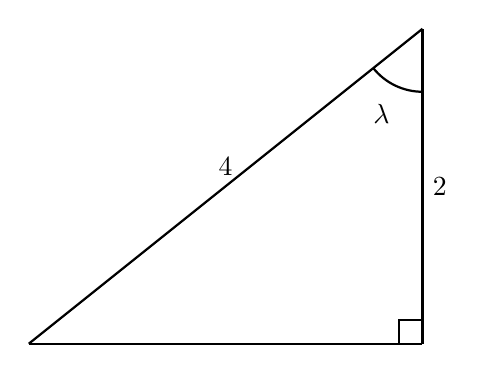
\begin{tikzpicture}[thick]
          \coordinate (A) at (0,1);
          \coordinate (B) at (5,5);
          \coordinate (C) at (5,1);

          \draw[black] (5,1) -- (5,5) node[midway, right]{$2$};
          \draw[black] (0,1) -- (5,1);
          \draw (4.7,1) |- ++(0.3,0.3);
          \draw[black] (0,1) -- (5,5) node[midway, above]{$4$};

          \tkzMarkAngle[fill= orange,size=0.8cm,%
          opacity=1](A,B,C)
          \tkzLabelAngle[pos = 1.2](A,B,C){$\lambda$}

          \end{tikzpicture}

      \task \texttt{(**)}\\
          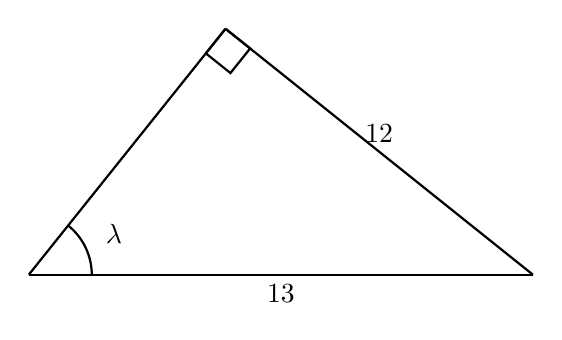
\begin{tikzpicture}[thick]
          \coordinate (Q) at (0,2);
          \coordinate (R) at (2.49878019,5.123475);
          \coordinate (P) at (6.403124,2);

          \draw[black] (0,2) -- (6.403124,2) node[midway, below]{$13$};
          \draw[black] (0,2) -- (2.49878019,5.123475);
          \draw[black] (6.403124,2) -- (2.49878019,5.123475) node[midway, above, inner sep=3pt]{12};
          \draw[black] (0,2) {};

          \tkzMarkRightAngle[size=0.4,opacity=1](Q,R,P)% square angle here

          \tkzMarkAngle[fill= orange,size=0.8cm,%
          opacity=1](P,Q,R)
          \tkzLabelAngle[pos = 1.2](P,Q,R){$\lambda$}

          \end{tikzpicture}

    \end{tasks}
  \end{ex}









  

	\end{lec}

\end{document}




















































